\documentclass{standalone}
\usepackage{mintikz}
\usepackage{schemabloc}

% \newlength{\nodedistance}
% \settowidth{\nodedistance}{3cm}
\begin{document}
\begin{tikzpicture}[%
		every node/.style={draw, rounded corners, align=center},
		meca/.style={%
				fill=mygreen, opacity=.5,
				text opacity=1, draw opacity=1%
			},
		elec/.style={%
				fill=myblue, opacity=.5,
				text opacity=1, draw opacity=1%
			},
	]
	\tikzset{node distance={4cm}}
	\node[elec] (C) at (0,0) {Courant};
	\node[right of=C] (L) {Force de\\\textsc{Laplace}};
	\node[meca, right of=L] {Mouvement\\du circuit};
\end{tikzpicture}

\begin{tikzpicture}[auto,
	node distance=2,
	start chain=A going right,
	meca/.style={%
			fill=mygreen, opacity=.5,
			text opacity=1, draw opacity=1%
		},
	elec/.style={%
			fill=myblue, opacity=.5,
			text opacity=1, draw opacity=1%
		},
	block/.style={draw, rounded corners, align=center,
			minimum height=11mm, minimum width=12mm,
			on chain=#1, join},
	block/.default=A,
	sum/.style n args={5}{circle, draw, minimum size=9mm,
			append after command={\pgfextra{\let\LN\tikzlastnode}
					(\LN.north west) edge (\LN.south east)
					(\LN.south west) edge (\LN.north east)
					node[left]     at (\LN.center) {$#2$}
					node[above]    at (\LN.center) {$#3$}
					node[right]    at (\LN.center) {$#4$}
					node[below]    at (\LN.center) {$#5$}
				},
			node contents={},
			on chain=#1, join},
	sum/.default={A}{+}{+}{}{},
	arr/.style={-{Stealth[scale=1]}, semithick},
	every edge quotes/.style={inner sep=2pt},
	every join/.style={-{Stealth[scale=1]}, semithick}
	]
	\begin{scope}
		\node[block, elec] (in) {Courant};                   % A-1
		\tikzset{node distance={1cm}}
		\node[sum={A}{+}{}{}{-}];                       % A-2
		\node[sum={A}{+}{+}{}{}];                       % A-3
		\tikzset{node distance={2cm}}
		\node[block] {\textsc{Laplace}}; % A-4
		\node[above]
		at ($(A-3)!0.45!(A-4)$)
		{action};
		\node[below]
		at ($(A-3)!0.45!(A-4)$)
		{mécanique};
		\tikzset{node distance={1.5cm}}
		\node[block, meca, join=by {"$\Ff\ind{Lap}$"}] {Mouvement}; % A-5
		\tikzset{node distance={1.5cm}}
		% \node[block, join=by {"$\dv{S}{t} \neq 0$"}] {$\DS \dv{\F}{t} \neq 0$}; % A-6
		\node[block, join=by {"$\DS \dv{\F}{t} \neq 0$"}] {$e\ind{ind}$}; % A-7
		% \node[block] {$i\ind{ind}$}; % A-8
		\node[block] {Courant\\induit};                     % A-8
		\draw[arr]
		(A-7) --++
		(0,-1) -|
		node[near end, right] {Lenz}
		(A-2);
		\node[above]
		at ($(A-6)!0.45!(A-7)$)
		{circuit};
		\node[below]
		at ($(A-6)!0.45!(A-7)$)
		{fermé};
	\end{scope}

	\node[start chain=B going below, block=B, above=1 of A-3,
		join=with A-3 by {{Stealth[scale=1]}-}%, "champ mag"}
	] {$\Bf\ind{ext}$};
	% \draw[arr]  (in)    edge ["Set point"]  (A-2)
	% (A-2)   edge ["$E(s)$"]     (A-3)
	% (A-3)   edge ["$u(s)$"]     (A-4)
	% (A-4)   edge ["Output"]     (out)
	% ($(A-4.east)!0.5!(out)$) -- ++ (0,-11mm)
	% -| (A-2);
\end{tikzpicture}

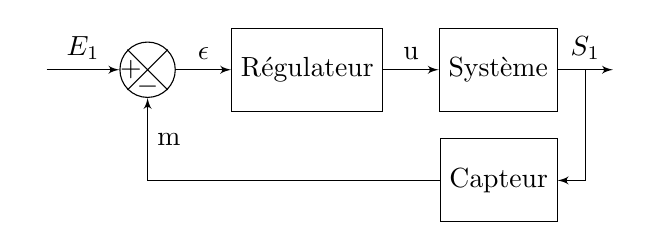
\begin{tikzpicture}
	\sbEntree{E}
	\sbComp{comp}{E}
	\sbRelier[$E_1$]{E}{comp}
	\sbBloc{reg}{Régulateur}{comp}
	\sbRelier[$\epsilon$]{comp}{reg}
	\sbBloc{sys}{Système}{reg}
	\sbRelier[u]{reg}{sys}
	\sbSortie{S}{sys}
	\sbRelier[$S_1$]{sys}{S}
	\sbDecaleNoeudy[4]{S}{U}
	\sbBlocr{cap}{Capteur}{U}
	\sbRelieryx{sys-S}{cap}
	\sbRelierxy[m]{cap}{comp}
\end{tikzpicture}

\begin{tikzpicture}
	\sbEntree{O}
	\sbStyleLien{semithick, -{Stealth[scale=1]}}
	\sbBloc[0]{I}{Courant}{O}
	\sbComp{Ilenz}{I}
	\sbSumh{IB}{Ilenz}
	\sbBloc{lap}{Laplace}{IB}
	\sbBloc{mvt}{Mouvement}{lap}
	\sbBloc{flux}{$\dv{\F}{t} \neq 0$}{mvt}
	\sbBloc{eind}{$e\ind{ind}$}{flux}
	\sbBloc{iind}{$i\ind{ind}$}{eind}
	\sbRenvoi{iind}{Ilenz}{Lenz}
\end{tikzpicture}

\end{document}
